\documentclass{report}

\oddsidemargin 0.0in
\evensidemargin 0.0in
\textwidth 6.5in

\title{SORTS Tech Report}
\author{James Irizarry, Sam Wintermute, Joseph Xu}

\begin{document}
\maketitle

\section{ORTS Overview}

The Open Real Time Strategy software is a highly configurable game
engine used to play real time strategy (RTS) games \cite{ORTS}. The main
purpose for ORTS is to serve as an open source, open interface RTS game
engine for RTS AI tournaments. ORTS is undergoing active development as
of July 2006 at the University of Alberta under the direction of Michael
Buro.

There are several reasons why ORTS is especially suitable for use in
AI tournaments. It has a (relatively) straightforward C++ API, making
interfacing with your favorite AI system easy. All the specific game
mechanics, ranging from types of units, actions, and physics, are
specified via C++ style scripts called blueprints. This means that ORTS
can be easily configured to simulate a wide range of environments,
from arbitrarily simple ones like Wumpus World to complex ones like
Starcraft. Finally, ORTS has a client/server architecture in which
the server maintains the state of the world and only report to the
clients information they are supposed to have for a fair game. This
is in contrast to most commercial RTS games, in which each client
maintains the entire world state and prevents the player from accessing
forbidden information such as other players' locations only by hiding
them from the GUI. The result is that ORTS is impervious to "memory
hack" cheats that are widespread in commercial RTS games. This feature
is particularly important if tournaments are to be run across the
Internet.

\section{SORTS Overview}

SORTS is a piece of software that allows the Soar cognitive architecture
to act as a client to the ORTS game server, so that ORTS game playing
agents can be written in and executed on Soar. SORTS is much more than
an interface bridge in that it intentionally constrains the space of
possible Soar agents in important ways and also handles aspects of
low-level game control that are not suitable for Soar. In particular,
SORTS heavily abstracts the world state information obtained from
the ORTS API before feeding them into Soar as perceptions, and also
interprets and executes high-level commands from Soar as low-level
actions sent to the ORTS API.

\section{Updating the Game State}

\subsection{Raw State Information}

The ORTS API provides complete game state update information in the form
of 6 lists:

\begin{itemize}
  \item \verb|new_tile_indexes| New game tiles encountered via
  uncovering of fog of war.
  \item \verb|new_objs| New game objects, such as enemy units and
  buildings, or world objects such as trees.
  \item \verb|changed_objs| Game objects that have changed since the
  previous viewframe.
  \item \verb|vanished_objs| Game objects that disappeared from the
  player's vision.
  \item \verb|dead_objs| Game objects that died.
  \item \verb|new_boundaries| New terrain boundaries that demarcate
  the border between different terrain types, such as ground and cliff.
\end{itemize}

SORTS currently takes into account the information in all
the lists except \verb|new_tile_indexes| and
\verb|new_boundaries|. The former is ignored because SORTS
currently does not have any functioning capability to reason about
terrain, except for collision detection. The latter is ignored because
we get this information from the game tiles directly whenever we check
for boundaries. Note also that currently, SORTS treats objects vanishing
(reported in \verb|vanished_objs|) and objects dying (reported in
\verb|dead_objs|) as one and the same thing. This will probably change
in the future as agents use more sophisticated reasoning.

All game state updates, both internal to the middleware and to the Soar
input link, are performed in the ORTS event handler, which is triggered
everytime the middleware receives a new viewframe from the ORTS server.
An overview of the flow of control among the various functions is shown
in figure~\ref{fig:flow}. Detailed descriptions of the two event
handlers are provided below.

\begin{figure}
\includegraphics[width=\textwidth]{graphics/flow.eps}
\caption{Overview of how control is passed through Sorts. Note that the
two gray regions represent two different threads executing
asynchronously.}
\label{fig:flow}
\end{figure}

\subsection{The ORTS Event Handler}
\label{sec:OrtsEventHandler}

The ORTS event handler is triggered everytime the middleware receives
a new viewframe from the ORTS server. This event handler and the
Soar event handler are the main functions from which most other
function calls are made. Pseudo-code for the handler is shown in
figure~\ref{fig:OrtsEventHandler}.

\begin{figure}
\begin{verbatim}
ORTSEventHandler
  lockMutex()
  mergeChanges(oldChanges, changes)
  if currentViewFrame - lastActionFrame > ALLOWED_LAG then
    unlockMutex()
    return
  end
  removeDeadObjects(changes)
  assignSoarActions()
  updateSoarGameObjects(changes)
  sendActions()
  updateGroups()
  unlockMutex()
end
\end{verbatim}
\caption{Pseudo code for the ORTS event handler}
\label{fig:OrtsEventHandler}
\end{figure}

Each function call is described below.

\begin{itemize}

\item \verb|lockMutex()| and \verb|unlockMutex()|
  This mutex locks the Soar event handler from executing until the
  ORTS event handler is finished. This is important since we don't want
  the Soar command buffer to change while we are processing that buffer.

\item \verb|mergeChanges(oldChanges, changes)|
  If SORTS falls behind the ORTS server too much, changes to the game
  state will be accumulated but not processed in the interest of
  catching up. This function merges changes reported in previous
  viewframes with the current changes.

\item \verb|removeDeadObjects(changes)|
  This function removes all game objects that have just died or vanished
  in the current frame. This call needs to be made before the call to
  \verb|assignSoarActions()| so that we don't try to assign any actions
  to objects that disappeared, which the ORTS server would not
  understand.

\item \verb|assignSoarActions()|
  Interprets commands queued from the Soar output-link as ORTS actions and
  distributes them to the appropriate groups. The actions are not sent
  to the ORTS server until \verb|sendActions()| is called.

\item \verb|updateSoarGameObjects(changes)|
  This is the main function that updates the attributes of the
  SoarGameObject structures in the middleware. It is called after
  \verb|assignSoarActions()| so that units will begin responding to
  their commands in the Soar cycle that immediately follows the one in
  which they were assigned.

\item \verb|sendActions()|
  This is a call to the ORTS API that sends all queued actions to the
  server.

\item \verb|updateGroups()|
  Runs the grouping algorithm over SoarGameObjects that have changed or
  appeared, and prunes those groups whose members have died. These
  changes are directly reflected in the Soar input-link, but are
  buffered in the SML interface until the next Soar decision cycle.

\end{itemize}

\subsection{The Soar Event Handler}
\label{sec:SoarEventHandler}

The Soar event handler is triggered at the end of each Soar decision
cycle. The main responsibility of this function is to take commands off
the Soar output-link and buffer them into action queues in the
middleware.

\begin{figure}
\begin{verbatim}
SoarEventHandler
  lockMutex()
  if Catchup = true then
    unlockMutex()
    return
  end if
  getNewSoarOutput()
  processVisionCommands()
  processGameCommands()
  unlockMutex()
end
\end{verbatim}
\caption{Pseudo code for the Soar event handler}
\label{fig:SoarEventHandler}
\end{figure}

Figure~\ref{fig:SoarEventHandler} shows the pseudo-code for the
function. The following is a list of descriptions for each call made in
the function.

\begin{itemize}

\item \verb|lockMutex()| and \verb|unlockMutex()|
  These calls lock on the same mutex as the ORTS event handler, thereby
  making the execution of these two functions mutually exclusive.

\item \verb|getNewSoarOutput()|
  Takes all commands on the Soar output-link and queues them into lists
  in the middleware. This includes both commands issued to in-game units
  as well as commands that adjust middleware parameters such as grouping
  radius and center of visual attention. However, none of the commands
  are actually processed by this function.

\item \verb|processVisionCommands()|
  Processes Soar commands related to the perceptual system. These
  commands include changing the grouping radius, looking at a specific
  coordinate, looking at a feature in the feature map, and changing the
  maximum number of objects allowed on the input-link at any time (for
  a complete list, see section~\ref{sec:output-link}. These commands
  are processed here rather than with the in-game commands because Soar decision cycles can occur much faster than ORTS events.

\item \verb|processGameCommands()|
  Handles all commands that affect the way the middleware executes
  low-level actions, such as in the FSMs, but do not translate directly
  into ORTS game object actions. Also handles miscellaneous queries that
  Soar may make to the middleware for information not normally provided
  to it. Currently, there are only three such commands: finding a
  location for a building, and setting and clearing the mineral buffer
  (see section~\ref{sec:output-link}).

\end{itemize}



\section{Soar IO Description}

\subsection{The SORTS input-link}

There are five top-level attributes on the SORTS input link, "groups", "game-info", "feature-maps", "vision-info", and "query-results". The groups, feature-maps, and vision-info structures are all part of the main visual system (see XXX), while game-info contains higher-level information about the game world, and query-results is used to communicate the results of specialized queries from Soar to the middleware.

The exact data structures are as follows:

\begin{center}
\begin{tabular}{|l|p{4.0in}|}
\hline
\multicolumn{2}{|c|}{\textbf{Attributes of io.input-link}}\\ 
\hline
attribute  &  description\\
\hline \hline
\multicolumn{2}{|l|}{\textbf{vision-info structure:}}\\ 
\hline
vision-info & Contains information on the current state of the vision system. \\
\hline
vision-info.center-x & The coordinate of the center of the region in view. \\
vision-info.center-y & \\
\hline
vision-info.focus-x & The coordinate of the center of focus (spotlight of attention). \\
vision-info.focus-y & \\
\hline
vision-info.num-objects-visible & The maximum number of objects (groups) present on the input-link. All other objects within the view window are present in feature maps. \\
\hline
vision-info.grouping-radius & All objects of the same type (except as below) and owner within this distance of each other are in the same group (set to 0 for individuals). \\
\hline
vision-info.owner-grouping & Ignore type when grouping, only group by owner (1 if enabled, 0 if disabled). \\
\hline
\multicolumn{2}{|l|}{\textbf{groups structure:}}\\ 
\hline
groups & The set of groups being attended to. \\
\hline
groups.group & Multi-valued, one instance for each group. Detailed below. \\
\hline
\multicolumn{2}{|l|}{\textbf{feature-maps structure:}}\\ 
\hline
feature-maps & Contains all feature maps- low-resolution information about certain features of unattended (but visible) objects. \\
\hline
feature-maps.friendly & Friendly feature map- each friendly unit (not group) results in one instance of this feature, marked in the sector of the group's center of gravity. \\
\hline
feature-maps.friendly-workers & A subset of the friendly feature map, showing only workers.\\
\hline
feature-maps.enemy & Similar to the above, but for enemy units.\\
\hline
feature-maps.minerals & Similar to the above, but for minerals.\\
\hline
feature-maps.moving-units & Moving units (if grouping is used, one moving object causes the whole group to be seen as moving).\\
\hline
feature-maps.(any).sector0 & Feature counts for each of the nine sectors. 0 is the upper left, 8 is the lower right.\\
.. & \\
feature-maps.(any).sector8 & \\
\hline
\multicolumn{2}{|l|}{\textbf{game-info structure:}}\\ 
\hline
game-info & General information about the game (non-visual information).\\
\hline
game-info.num-players & The number of players.\\
\hline
game-info.player-id & The ID number of the Soar player.\\
\hline
game-info.map-xdim & The dimensions of the game map. \\
game-info.map-ydim & \\
\hline
game-info.view-frame & The last view frame handled by the middleware (the number of game cycles executed).\\
\hline
game-info.my-minerals & Minerals available to the player. \\
\hline
game-info.mineral-buffer & The number of minerals to reserve for certain tasks (see section XXX).\\
\hline
game-info.worker-count & The number of units of each type owned by the player. \\
game-info.marine-count & \\
game-info.tank-count & \\
\hline
\multicolumn{2}{|l|}{\textbf{query-results structure:}}\\ 
\hline
query-results & The result of the last query to the middleware.\\
\hline
query-results.query-name & The name of the last query executed.\\
\hline
query-results.param0 & Query return values- the meaning of these is dependant on the query-name. \\
query-resutls.param1 & \\
\hline

\end{tabular}

\begin{tabular}{|l|l|p{3.5in}|}
\hline
\multicolumn{3}{|c|}{\textbf{Attributes of io.input-link.groups.group objects}}\\ 
\hline
attribute  & which groups &  description\\
\hline \hline
num-members & all & The number of individuals comprising the group. \\
\hline
type & all &The type of the group (ex: worker, mineral). \\
\hline
x-pos & all &The x,y location of the center of gravity of the group.\\
y-pos & & \\
\hline
x-min & all &The bounding box of the group.\\
x-max & & \\
y-min & & \\
y-max & & \\
\hline
health & all &The sum of the health of all units in the group.\\
\hline
taking-damage & all &The number of members of the group currently taking damage (under attack). \\
\hline
shooting & all &The number of members of the group currently attacking an enemy. \\
\hline
speed & all &The average speed of the group. \\
\hline
heading & all &The average heading of the group. \\
\hline
dist-to-focus & all &The distance from the center of gravity of the group to the attentional focus point.\\
\hline
dist-to-query & all &The distance from the center of gravity of the group to the last query location.\\
\hline
owner & all &The player number of the group's owner.\\
\hline
enemy & all &1 if the group belongs to an enemy player, 0 otherwise.\\
\hline
sticky & friendly & 1 if the group is sticky- sticky groups remain together even if they are no longer spatially close.\\
\hline
command & friendly & The last command issued to the group ("none" if no command has been issued).\\
\hline
command-running & friendly & The number of members of the group currently executing a command.\\
\hline
command-success & friendly & The number of members of the group that successfully completed the last command.\\
\hline
command-failure & friendly & The number of members of the group that unsuccessfully completed the last command.\\
\hline
minerals & friendly workers & The total number of minerals possessed by the workers in the group.\\
\hline
active-mining & friendly workers & The number of workers that are actively mining.\\
\hline
\end{tabular}
\end{center}

\subsection{The SORTS output-link}

The output-link allows the Soar agent to act in the game world by issuing commands to groups of friendly units, communicate directly to the middleware for actions such as querying,
and adjust the parameters of the visual subsystem in the middleware. All structures on the output link are similar- the Soar agent creates an output-link.command object with a name (\textbf{output-link.command.name}) specified. Depending on the command name, different parameters are needed. Parameters are attached to the command structure, as in \textbf{output-link.command.param0}. All legal commands and their necessary parameters are detailed below.


\begin{center}
\begin{minipage}{6.5in}
\begin{tabular}{|l|p{1.0in}|p{3.5in}|}
\hline
\multicolumn{3}{|c|}{\textbf{Soar output-link commands}}\\ 
\hline
command name &  parameters & description \\
\hline \hline
\multicolumn{3}{|l|}{\textbf{Vision commands}}\\ 
\hline
grouping-radius & $value$ & Change the grouping radius of the vision system. \\
\hline
enable-owner-grouping & (none) & Enable grouping-by-owner.\\
\hline
disable-owner-grouping & (none) & Disable grouping-by-owner.\\
\hline
change-view-width & $value$ & Change the width of the agent's view to be $value$.\\
\hline 
look-at-location & $x,y$ & Move the focus of attention to the given coordinate (which must be in the current view window.\\
\hline
move-to-location & $x,y$ & Shift the view window to be centered at the given coordinate, and make that the focus of attention. \\
\hline
look-at-feature & $feature$, $sector$ & Move the focus of attention to a given feature in a given sector. The legal features are the names of the feature-map objects on the input link.\\
\hline
move-to-feature & $feature$, $sector$ & As above, but re-center the view window to the new location, also.\\
\hline
num-objects & $value$ & Change the maximum number of objects (groups) present on the input-link at once.\\
\hline
\multicolumn{3}{|l|}{\textbf{General middleware commands}}\\ 
\hline
locate-building & $building$, $x,y$, $distance$ & This command requests that the middleware attempt to find a location for a building of type $building$ approximately $distance$ units from the coordinate given. The resulting coordinate is returned through the query-result structure on the input-link. \\
\hline
increase-mineral-buffer & $value$ & Increase the mineral buffer by $value$ minerals.\\
\hline
clear-mineral-buffer & (none) & Set the mineral buffer to 0.\\
\hline
\multicolumn{3}{|l|}{\textbf{Group commands}}\\
\hline
move & $group0$, $param0$, $param1$ & Move the group with ID $group0$ to the x,y location where $param0$ is x and $param1$ is y, using the default precision of 10 (allow units to complete successfully if they are within 10 of the target).\\
\hline
move & $group0$, $param0$, $param1$, $param2$ & Move group $group0$ to the x,y location where $param0$ is x and $param1$ is y, using a precision of $param2$.\\
\hline
build & $group0$, $param0 .. param3$ & Use group $group0$ to build a building of type $param0$\footnote{Legal building types: 0=controlCenter, 1=barracks, 2=factory} at the x,y location given by $param1, param2$. If $param3$ is 1, the mineral buffer is used, otherwise it is not. \\
\hline
train & $group0$, $param0 .. param2$ & Use group $group0$ (a building) to train units of type $param1$\footnote{Legal unit types: 0=worker, 1=marine, 2=tank}. Train up to $param2$ units, and use the mineral buffer if $param3$ is 1. \\
\hline
attack & $group0$, $group1$ & Use the friendly group with ID $group0$ to attack $group1$.\\
\hline
mine & $group0$ & Assign $group0$ to mine minerals. The control center and mineral patch to use are automatically determined in the middleware. \\
\hline
stick & $group0$ & Set $group0$'s to be sticky- ensure it stays as one group, even if the members move apart. Assigning any of the above actions to a group does this by default. \\
\hline
free & $group0$ & Clear $group0$'s sticky status- allow the members to be split up and join other groups.\\
\hline
join &  $group0$, $group1$ & Force $group0$'s members to join $group1$. If $group1$ is not sticky, this may be automatically undone the next cycle.\\
\hline
\end{tabular}
\end{minipage}
\end{center}


\bibliographystyle{plain}
\bibliography{report}

\end{document}
